%=========================================================================
% (c) 2011, 2012 Josef Lusticky

\chapter{Protothreads Example}\label{app:protothreads}
Listing~\ref{lst:app-protothreads-example} shows
an example of delaying text on an LCD panel using Protothreads.
It is taken from
Adam Dunkels' Protothreads website~\cite{adam-protothreads} and slightly modified.
Protothreads can be used to introduce delays inside a function without using a full threading model.
The example shows a function writing characters to an LCD panel.
Suppose that each character is shown for one second, then the next character replaces the previous.
\begin{lstlisting}[numbers=left,caption={Example using Protothreads},label=lst:app-protothreads-example]
#include "pt.h"
#include "timer.h"
#include <string.h>

typedef unsigned short lc_t;
struct pt {
  lc_t lc;                                           /* Local continuation */
};

struct pt state;
struct timer timer;

PT_THREAD(display_text(struct pt *pt, const char *msg))
{
  PT_BEGIN(pt);
  for (int i = 0; i < strlen(msg); i++) {
    lcd_display_char(msg[i]);
    timer_set(&timer, CLOCK_SECOND);               /* Wait for one second. */
    PT_WAIT_UNTIL(pt, timer_expired(&timer));
  }
  PT_END(pt);
}

int main(void)
{
  PT_INIT(&state);
  for (;;) {
    display_text(&state, "Hello world");
    /* Here could be another thread run */
  }
  return 0;
}
\end{lstlisting}
%\newpage
The PT\_WAIT\_UNTIL macro actually causes the function to return.
While the function is waiting for the timer to expire another function could be called and run.
When the function is entered again, the execution continues with the PT\_WAIT\_UNTIL macro
which causes the function to check the condition it is waiting for (timer expired).
If the condition is met, the function resumes, and it returns again if not.
Strictly speaking, the amount of time between showing each character can
be more than one second.
This is because Protothreads are not running simultaneously: if the timer expired
and another Protothread was running, this Protothread would have to wait until
it is entered again.
When the condition specified in PT\_WAIT\_UNTIL is met,
the next iteration of the {\it{for}} loop (line 16) is started and the next character is displayed.

How does it work? The macro PT\_BEGIN is expanded to a {\it switch} statement
by the preprocessor.
The PT\_WAIT\_UNTIL macro expands to {\it case} and setting the local continuation
to the value, so that the next time this function is run, it jumps to this {\it case}.
The structure holding the state is defined outside of the function, so its context is not lost when
the function returns. The simplest state structure would hold just the local continuation variable.
Listing~\ref{lst:app-protothreads-preprocessed} shows
the same example after a simplified preprocessing.
%\newpage
\begin{lstlisting}[numbers=left,caption={Preprocessed example using Protothreads},label=lst:app-protothreads-preprocessed]
#include "pt.h"
#include "timer.h"
#include <string.h>

typedef unsigned short lc_t;
struct pt {
  lc_t lc;                                           /* Local continuation */
};

struct pt state;
struct timer timer;

int display_text(struct pt *pt, const char *msg)     /* Expanded PT_THREAD */
{
  switch(pt->lc) {  case 0:                      /* Expanded PT_BEGIN(pt); */
    for (int i = 0; i < strlen(msg); i++) {
      lcd_display_char(msg[i]);
      timer_set(&timer, CLOCK_SECOND);             /* Wait for one second. */

                                   /* The following two lines are expanded */
      pt->lc = 31; case 31:   /* PT_WAIT_UNTIL(pt, timer_expired(&timer)); */
      if(!(timer_expired(&timer))) { return PT_WAITING; }         /* macro */

    }
  pt->lc = 0; return PT_ENDED; }                        /* Expanded PT_END */
}

int main(void)
{
  state->lc = 0;                                       /* Expanded PT_INIT */
  for (;;) {
    display_text(&state, "Hello world");
    /* Here could be another thread run */
  }
  return 0;
}
\end{lstlisting}


\chapter{Clock Interrupt Frequency Measurements}\label{app:interrupt-frequency}
\begin{figure}[H]
  \centering
  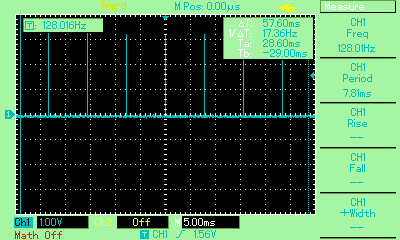
\includegraphics[width=10cm,keepaspectratio]{fig/osc-no-adjust.png}
  \caption{Interrupt frequency without clock adjustment}
  \label{fig:app-osc-no-adjust}
  \bigskip
\end{figure}

\begin{figure}[H]
  \centering
  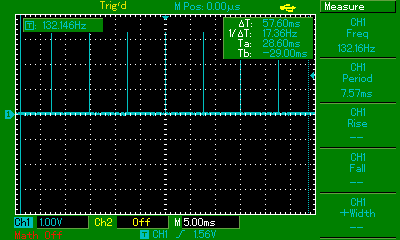
\includegraphics[width=10cm,keepaspectratio]{fig/osc-speed-up.png}
  \caption{Interrupt frequency when speeding up the clock}
  \label{fig:app-osc-speed-up}
  \bigskip
\end{figure}

\begin{figure}[H]
  \centering
  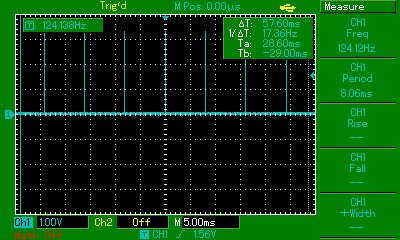
\includegraphics[width=10cm,keepaspectratio]{fig/osc-slow-down.png}
  \caption{Interrupt frequency when slowing down the clock}
  \label{fig:app-osc-slow-down}
  \bigskip
\end{figure}


\chapter{Clock Offset Measurements}\label{app:offset}
The serial output from AVR~Raven,
the TechTools~DigiView~DV3100 logic analyser and the Meinberg~GPS~167 clock
were used for measuring the local clock offset.
Meinberg~GPS~167 rises an impulse when each second is accounted.
AVR~Raven was configured to write a logic~1
to~bit~7 of~Port~D when each second is accounted,
and to write a logic~0 to~the same bit after~25 clock ticks.

Figure~\ref{fig:app-ntp-set-time} shows the local clock offset from long-term uptime
observation when NTP client sets the time, but no adjustments are applied.
A linear offset increase can be observed, until the threshold value
for setting the time is reached.
The offset threshold value was 3 seconds.
\begin{figure}[H]
  \centering
  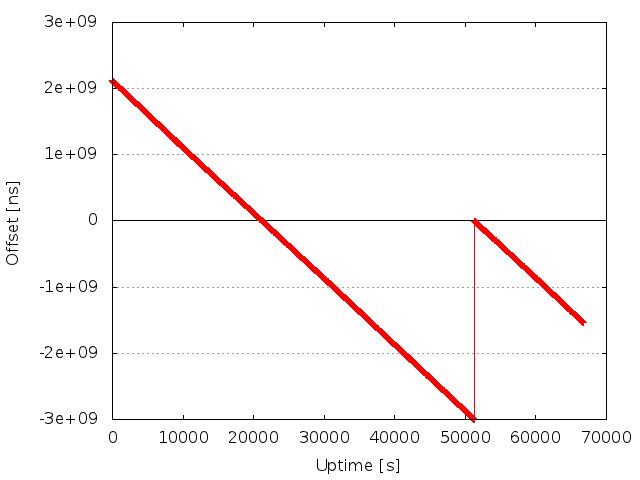
\includegraphics[width=11cm,keepaspectratio]{fig/set-time-3s.png}
  \caption{Local clock offset with NTP client setting the time but without adjustments}
  \label{fig:app-ntp-set-time}
\end{figure}

Figure~\ref{fig:app-ntp-la} shows the local clock offset
acquired from logic analyser when the Contiki NTP Client runs on the device.
The logic analyser captures the rising and the falling edge
from the Meinberg~GPS clock and from AVR~Raven.
The difference between the rising edge from
Meinberg~GPS clock and the rising edge from AVR~Raven gives the local clock offset.
\begin{figure}[H]
  \centering
  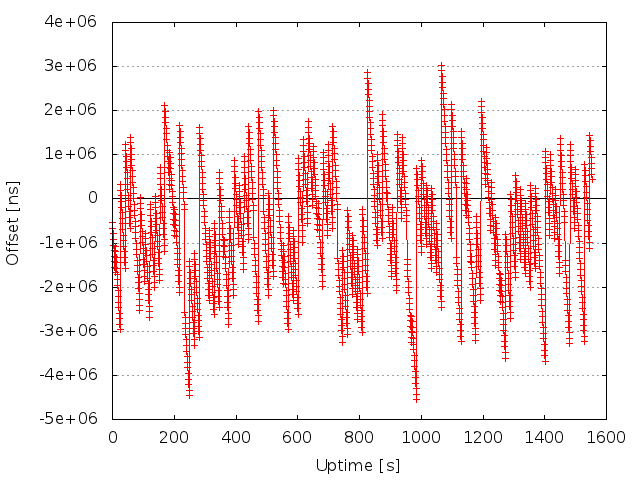
\includegraphics[width=11cm,keepaspectratio]{fig/la.png}
  \caption{Local clock offset with adjustments and NTP poll interval 16s}
  \label{fig:app-ntp-la}
\end{figure}


\chapter{Clock Phase Measurements}\label{app:phase}
The following figures show the phase difference between
the reference clock (Meinberg GPS 167) and AVR Raven.
The figures were acquired from the UNI-T 2025CEL digital oscilloscope.
The yellow line on~channel~2 shows the impulses from the GPS synchronised clock Meinberg GPS 167.
The blue line on~channel~1 shows the impulses from AVR Raven running
Contiki~OS with the developed NTP client.
The rising edge occurs when each second is being accounted.
Figure~\ref{fig:app-osc-out-of-phase} shows the clock out of phase
and figure~\ref{fig:app-osc-in-phase} shows the clock in phase.
\begin{figure}[ht]
  \centering
  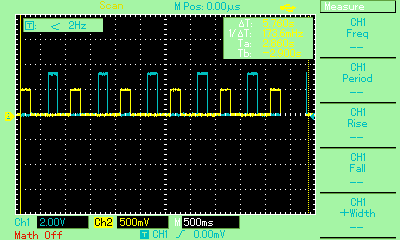
\includegraphics[width=11cm,keepaspectratio]{fig/osc-out-of-phase.png}
  \caption{Second impulses when the clock is out of phase}
  \label{fig:app-osc-out-of-phase}
  \bigskip
\end{figure}

\begin{figure}
  \centering
  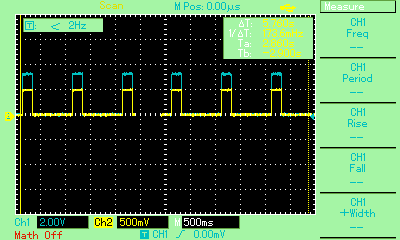
\includegraphics[width=11cm,keepaspectratio]{fig/osc-in-phase.png}
  \caption{Second impulses when the clock is in phase}
  \label{fig:app-osc-in-phase}
  \bigskip
\end{figure}


\chapter{CD Contents}\label{app:cd-contents}
\begin{tabular}{|l|l|}
	\hline
	Directory & Contents \\ \hline
	docs/ & Setup guides for running and debugging Contiki OS on AVR Raven\\
	docs/datasheets/ & Datasheets for used hardware\\
	docs/img/ & Images from Dopsy group laboratory at RheinMain University\\
	sw/ & Software used in this thesis including Contiki source code and patches\\
	sw/ntpd/ & Contiki NTP Client source code\\
	sw/utils/plots/ & Scripts and measured results for plots\\
	sw/utils/tests/ & Programs used for testing Contiki NTP Client\\
	text/ & LaTeX source files of this thesis\\
	text/fig/ & Figures used in this thesis\\
	\hline
\end{tabular}
